% Compile from docs/latex with XeLaTeX. Shared formatting: common.tex.
% Options for packages loaded elsewhere
\PassOptionsToPackage{unicode}{hyperref}
\PassOptionsToPackage{hyphens}{url}
\documentclass[
  11pt,
]{article}
\usepackage{xcolor}
\usepackage[margin=1in]{geometry}
\usepackage{amsmath,amssymb}
\setcounter{secnumdepth}{-\maxdimen} % remove section numbering
\usepackage{iftex}
\ifPDFTeX
  \usepackage[T1]{fontenc}
  \usepackage[utf8]{inputenc}
  \usepackage{textcomp} % provide euro and other symbols
\else % if luatex or xetex
  \usepackage{unicode-math} % this also loads fontspec
  \defaultfontfeatures{Scale=MatchLowercase}
  \defaultfontfeatures[\rmfamily]{Ligatures=TeX,Scale=1}
\fi
\usepackage{lmodern}
\ifPDFTeX\else
  % xetex/luatex font selection
  \IfFontExistsTF{Times New Roman}{\setmainfont{Times New Roman}}{\setmainfont{TeX Gyre Termes}}
\fi
% Use upquote if available, for straight quotes in verbatim environments
\IfFileExists{upquote.sty}{\usepackage{upquote}}{}
\IfFileExists{microtype.sty}{% use microtype if available
  \usepackage[]{microtype}
  \UseMicrotypeSet[protrusion]{basicmath} % disable protrusion for tt fonts
}{}
\makeatletter
\@ifundefined{KOMAClassName}{% if non-KOMA class
  \IfFileExists{parskip.sty}{%
    \usepackage{parskip}
  }{% else
    \setlength{\parindent}{0pt}
    \setlength{\parskip}{6pt plus 2pt minus 1pt}}
}{% if KOMA class
  \KOMAoptions{parskip=half}}
\makeatother
\usepackage{longtable,booktabs,array}
\usepackage{caption}
\captionsetup[longtable]{position=bottom,skip=5pt,font={scriptsize,it},width=\linewidth,justification=centering}
\newcounter{none} % for unnumbered tables
\usepackage{calc} % for calculating minipage widths
% Correct order of tables after \paragraph or \subparagraph
\usepackage{etoolbox}
\makeatletter
\patchcmd\longtable{\par}{\if@noskipsec\mbox{}\fi\par}{}{}
\makeatother
\usepackage{graphicx}
\makeatletter
\newsavebox\pandoc@box
\newcommand*\pandocbounded[1]{% scales image to fit in text height/width
  \sbox\pandoc@box{#1}%
  \Gscale@div\@tempa{\textheight}{\dimexpr\ht\pandoc@box+\dp\pandoc@box\relax}%
  \Gscale@div\@tempb{\linewidth}{\wd\pandoc@box}%
  \ifdim\@tempb\p@<\@tempa\p@\let\@tempa\@tempb\fi% select the smaller of both
  \ifdim\@tempa\p@<\p@\scalebox{\@tempa}{\usebox\pandoc@box}%
  \else\usebox{\pandoc@box}%
  \fi%
}
% Set default figure placement to htbp
\def\fps@figure{htbp}
\makeatother
\setlength{\emergencystretch}{3em} % prevent overfull lines
\providecommand{\tightlist}{%
  \setlength{\itemsep}{0pt}\setlength{\parskip}{0pt}}
\usepackage{bookmark}
\IfFileExists{xurl.sty}{\usepackage{xurl}}{} % add URL line breaks if available
\urlstyle{same}
% fallback for those not using the hyperref driver hyperxmp:
\makeatletter
\@ifundefined{xmpquote}{\newcommand{\xmpquote}[1]{#1}}{}
\makeatother
\hypersetup{
  hidelinks,
  pdfcreator={LaTeX via pandoc}}



% Shared layout based on the Word test plan.
\usepackage{sectsty}
\sectionfont{\fontsize{14}{17}\selectfont}
\subsectionfont{\fontsize{12}{15}\selectfont}
\subsubsectionfont{\fontsize{11}{14}\selectfont}
\AtBeginEnvironment{longtable}{\fontsize{8.5}{10.5}\selectfont}
\newcommand{\projecttitle}[1]{\begin{center}{\fontsize{22}{26}\selectfont #1\par}\end{center}}
\newcommand{\documentsubtitle}[1]{\begin{center}{\fontsize{15}{18}\selectfont #1\par}\end{center}}

\renewcommand{\contentsname}{Table of Contents}
\makeatletter
\renewcommand*\l@section[2]{\@dottedtocline{1}{0em}{0em}{\textbf{#1}}{#2}}
\renewcommand*\l@subsection[2]{\@dottedtocline{2}{1.5em}{0em}{\normalfont #1}{#2}}
\makeatother


\begin{document}

\projecttitle{AI-Driven Pharmaceutical Real-Time Inventory and Customer Information System}

\documentsubtitle{Software Test Plan}

\begin{center}{\fontsize{12}{14}\selectfont\itshape Draft: Version 0.1\par}\end{center}

Course: Software Engineering

Team: Seal-SIMD

Team Members: Maria Molano Escobar, Marko Maksuti, Ryan Petillo, Samuel Cordova

Instructor: Hubert Johnson

Date: November 12, 2026

\clearpage
\section*{Revision History}

{\def\LTcaptype{none} % do not increment counter
\begin{longtable}[]{|
  >{\raggedright\arraybackslash}m{(\linewidth - 8\tabcolsep - 5\arrayrulewidth) * \real{0.2500}}|
  >{\raggedright\arraybackslash}m{(\linewidth - 8\tabcolsep - 5\arrayrulewidth) * \real{0.2500}}|
  >{\raggedright\arraybackslash}m{(\linewidth - 8\tabcolsep - 5\arrayrulewidth) * \real{0.2500}}|
  >{\raggedright\arraybackslash}m{(\linewidth - 8\tabcolsep - 5\arrayrulewidth) * \real{0.2499}}|}
\hline
\begin{minipage}[c]{\linewidth}\raggedright
\textbf{Version}
\end{minipage} & \begin{minipage}[c]{\linewidth}\raggedright
\textbf{Date}
\end{minipage} & \begin{minipage}[c]{\linewidth}\raggedright
\textbf{Author}
\end{minipage} & \begin{minipage}[c]{\linewidth}\raggedright
\textbf{Description}
\end{minipage} \\
\hline
\endhead

\endlastfoot
0.1 & Nov 12, 2026 & Seal-SIMD Team & Initial draft based on Week 10 assignment, SRS v0.3, and Week 8 detailed design. \\ \hline
\end{longtable}
}

\clearpage
\tableofcontents

\clearpage
\section{1. Introduction}\label{introduction}

\subsection{1.1. Purpose}\label{purpose}

This Software Test Plan defines how the Seal-SIMD team will verify and validate the AI-Driven Pharmaceutical Real-Time Inventory and Customer Information System. It translates the project requirements and detailed module design into a feasible sequence of unit, integration, functional, performance, reliability, security, and acceptance testing activities. The plan is intended both to demonstrate to course management that the system can be tested systematically and to provide the project team with concrete directions for the testing phase.

\subsection{1.2. Scope}\label{scope}

The planned tests cover the pharmacy operations application, customer information portal, shared backend services, persistent inventory data, machine-learning advisory functions, and external integration adapters defined in the Week 8 design. The plan emphasizes the core inventory kernel first, then integrates ordering, analytics, adapters, and customer-facing functionality. Out-of-scope product functions from the SRS - prescription dispensing, e-prescribing, insurance claims, online payment, home delivery, and medical or dosing advice - are not acceptance targets for this project version.

\subsection{1.3. Test Plan Organization}\label{test-plan-organization}

Section 2 states the overall objectives and success criteria. Section 3 defines and defends the integration strategy. Section 4 maps the required testing techniques to modules and describes methodology. Section 5 gives detailed planned test groups and acceptance criteria. Section 6 covers performance, reliability, security, and usability evaluation. Section 7 assigns proposed responsibilities and dates. Section 8 defines monitoring, defect reporting, regression, and correction procedures. Section 9 traces tests to requirements and modules. Section 10 describes acceptance and demonstration readiness.

\subsection{1.4. Glossary}\label{glossary}

{\def\LTcaptype{none} % do not increment counter
\begin{longtable}[]{|
  >{\raggedright\arraybackslash}m{(\linewidth - 4\tabcolsep - 3\arrayrulewidth) * \real{0.5001}}|
  >{\raggedright\arraybackslash}m{(\linewidth - 4\tabcolsep - 3\arrayrulewidth) * \real{0.4999}}|}
\hline
\begin{minipage}[c]{\linewidth}\raggedright
\textbf{Term}
\end{minipage} & \begin{minipage}[c]{\linewidth}\raggedright
\textbf{Definition}
\end{minipage} \\
\hline
\endhead

\caption*{Table 1.4.1. Test plan glossary}\\
\endlastfoot
API & Application Programming Interface \\ \hline
AI & Artificial Intelligence \\ \hline
CI & Continuous Integration \\ \hline
DSCSA & Drug Supply Chain Security Act \\ \hline
FEFO & First-Expired, First-Out \\ \hline
HIPAA & Health Insurance Portability and Accountability Act \\ \hline
I/O Testing & Input/output testing that validates accepted inputs, rejected inputs, and observable outputs \\ \hline
MAPE & Mean Absolute Percentage Error \\ \hline
MFA & Multi-Factor Authentication \\ \hline
ML & Machine Learning \\ \hline
NDC & National Drug Code \\ \hline
POS & Point of Sale \\ \hline
RBAC & Role-Based Access Control \\ \hline
Regression Test & Previously passed test rerun after a code or configuration change \\ \hline
SRS & Software Requirements Specification \\ \hline
System Under Test (SUT) & The integrated software product or component currently being tested \\ \hline
Test Oracle & The rule or expected result used to decide whether a test passes \\ \hline
Walkthrough & Structured peer examination of design, logic, interfaces, or test procedure \\ \hline
WCAG & Web Content Accessibility Guidelines \\ \hline
\end{longtable}
}

\clearpage
\section{2. Overall Objectives and Success Criteria}\label{overall-objectives-and-success-criteria}

\subsection{2.1. Overall Testing Objectives}\label{overall-testing-objectives}

\begin{itemize}
\item
  Verify that each module satisfies its exported interface, preconditions, postconditions, invariants, and error behavior defined by the detailed design.
\item
  Validate that the integrated system implements functional requirements F1-F25 without violating the stated safety, privacy, authorization, and human-approval constraints.
\item
  Demonstrate that stock updates are atomic, auditable, replay-safe, and never produce negative inventory or sell expired lots.
\item
  Confirm that customer-facing functionality exposes only safe public information, including coarse availability rather than exact stock quantities and protected handling of Schedule II products.
\item
  Evaluate the measurable non-functional targets for response time, update propagation, concurrency/scalability, availability/recovery, accessibility, automated coverage, and ML forecast quality where sufficient test data exists.
\item
  Provide repeatable evidence for the final acceptance demonstration and a documented process for defects, retesting, and regression.
\end{itemize}

\subsection{2.2. Global Success Criteria}\label{global-success-criteria}

{\def\LTcaptype{none} % do not increment counter
\begin{longtable}[]{|
  >{\raggedright\arraybackslash}m{(\linewidth - 4\tabcolsep - 3\arrayrulewidth) * \real{0.5001}}|
  >{\raggedright\arraybackslash}m{(\linewidth - 4\tabcolsep - 3\arrayrulewidth) * \real{0.4999}}|}
\hline
\begin{minipage}[c]{\linewidth}\raggedright
\textbf{Area}
\end{minipage} & \begin{minipage}[c]{\linewidth}\raggedright
\textbf{Initial-draft success criterion}
\end{minipage} \\
\hline
\endhead

\caption*{Table 2.2.1. Global test success criteria}\\
\endlastfoot
Functional correctness & All Must requirements have at least one planned test and no open Severity 1 defect at acceptance. \\ \hline
Inventory integrity & No test may produce negative lot quantity; every committed stock delta has an associated ledger/audit record; duplicate external events do not double-apply. \\ \hline
Authorization & Unauthorized role/store combinations are denied server-side; approval-only actions cannot be completed by a technician or customer. \\ \hline
Expiration safety & Expired lots are excluded from sellable stock and blocked from sale at execution time. \\ \hline
Public privacy & Customer search never reveals exact inventory quantity; Schedule II availability is replaced by the required contact-pharmacy message. \\ \hline
Performance & Customer search target: \textless=2 seconds under the defined test load; inventory changes visible system-wide within \textless=5 seconds. \\ \hline
Reliability & Offline store transactions are queued durably and synchronized on reconnect with no duplicate inventory effects; recoverable dependency failures do not corrupt inventory. \\ \hline
Automated coverage & Target \textgreater=70\% automated test coverage for implemented code, measured by the selected test framework. \\ \hline
Acceptance & All acceptance-demo scenarios complete with expected outputs or documented, instructor-approved limitations. \\ \hline
\end{longtable}
}

\subsection{2.3. Entry and Exit Criteria}\label{entry-and-exit-criteria}

{\def\LTcaptype{none} % do not increment counter
\begin{longtable}[]{|
  >{\raggedright\arraybackslash}m{(\linewidth - 6\tabcolsep - 4\arrayrulewidth) * \real{0.3333}}|
  >{\raggedright\arraybackslash}m{(\linewidth - 6\tabcolsep - 4\arrayrulewidth) * \real{0.3333}}|
  >{\raggedright\arraybackslash}m{(\linewidth - 6\tabcolsep - 4\arrayrulewidth) * \real{0.3333}}|}
\hline
\begin{minipage}[c]{\linewidth}\raggedright
\textbf{Stage}
\end{minipage} & \begin{minipage}[c]{\linewidth}\raggedright
\textbf{Entry criteria}
\end{minipage} & \begin{minipage}[c]{\linewidth}\raggedright
\textbf{Exit criteria}
\end{minipage} \\
\hline
\endhead

\caption*{Table 2.3.1. Stage entry and exit criteria}\\
\endlastfoot
Unit testing & Module compiles; interface contract defined; mocks/stubs available for required imports. & Planned critical unit cases pass; known failures logged; module ready for its next integration step. \\ \hline
Integration testing & Participating modules have completed critical unit cases; shared data contracts are stable. & Interface, transaction, and error-propagation cases pass; no unresolved blocking integration defect. \\ \hline
Functional/system testing & Core integrated path deployed in a controlled environment with representative synthetic data. & Must-requirement scenarios pass or have documented disposition; regression suite is green. \\ \hline
Performance/reliability & Functional baseline stable enough for repeatable measurements. & Targets measured and results recorded; material misses receive a defect or accepted limitation. \\ \hline
Acceptance & Final candidate build selected; critical defects resolved; demo data reset. & Demonstration scenarios completed and acceptance evidence packaged. \\ \hline
\end{longtable}
}

\clearpage
\section{3. Integration Plan}\label{integration-plan}

\subsection{3.1. Chosen Integration Strategy}\label{chosen-integration-strategy}

The project will use an incremental, dependency-driven integration strategy rather than a big-bang approach. Integration begins with identity/catalog foundations and the transactional inventory kernel because most later features depend on those contracts. Operational modules are then added around the kernel, followed by analytics and external adapters, and finally customer-facing and AI interaction modules. Stubs or mocks may represent external POS, supplier, map, mail, and ML dependencies until the corresponding adapter is ready. This keeps failures localized and allows each integration increment to be tested before another dependency is introduced.

\subsection{3.2. Integration Sequence and Defense}\label{integration-sequence-and-defense}

This order follows the dependency rules documented in the design: user interfaces call application services rather than the database; inventory mutations pass through the stock ledger; forecasting reads historical aggregates but does not write stock; and adapters use published integration ports. Testing the stock ledger and its callers early reduces the risk that later failures in dashboards, ordering, public search, or POS ingestion hide a transaction defect. Incremental integration also supports meaningful regression after each new module and makes it possible to continue testing with mocks when an external dependency is unavailable.

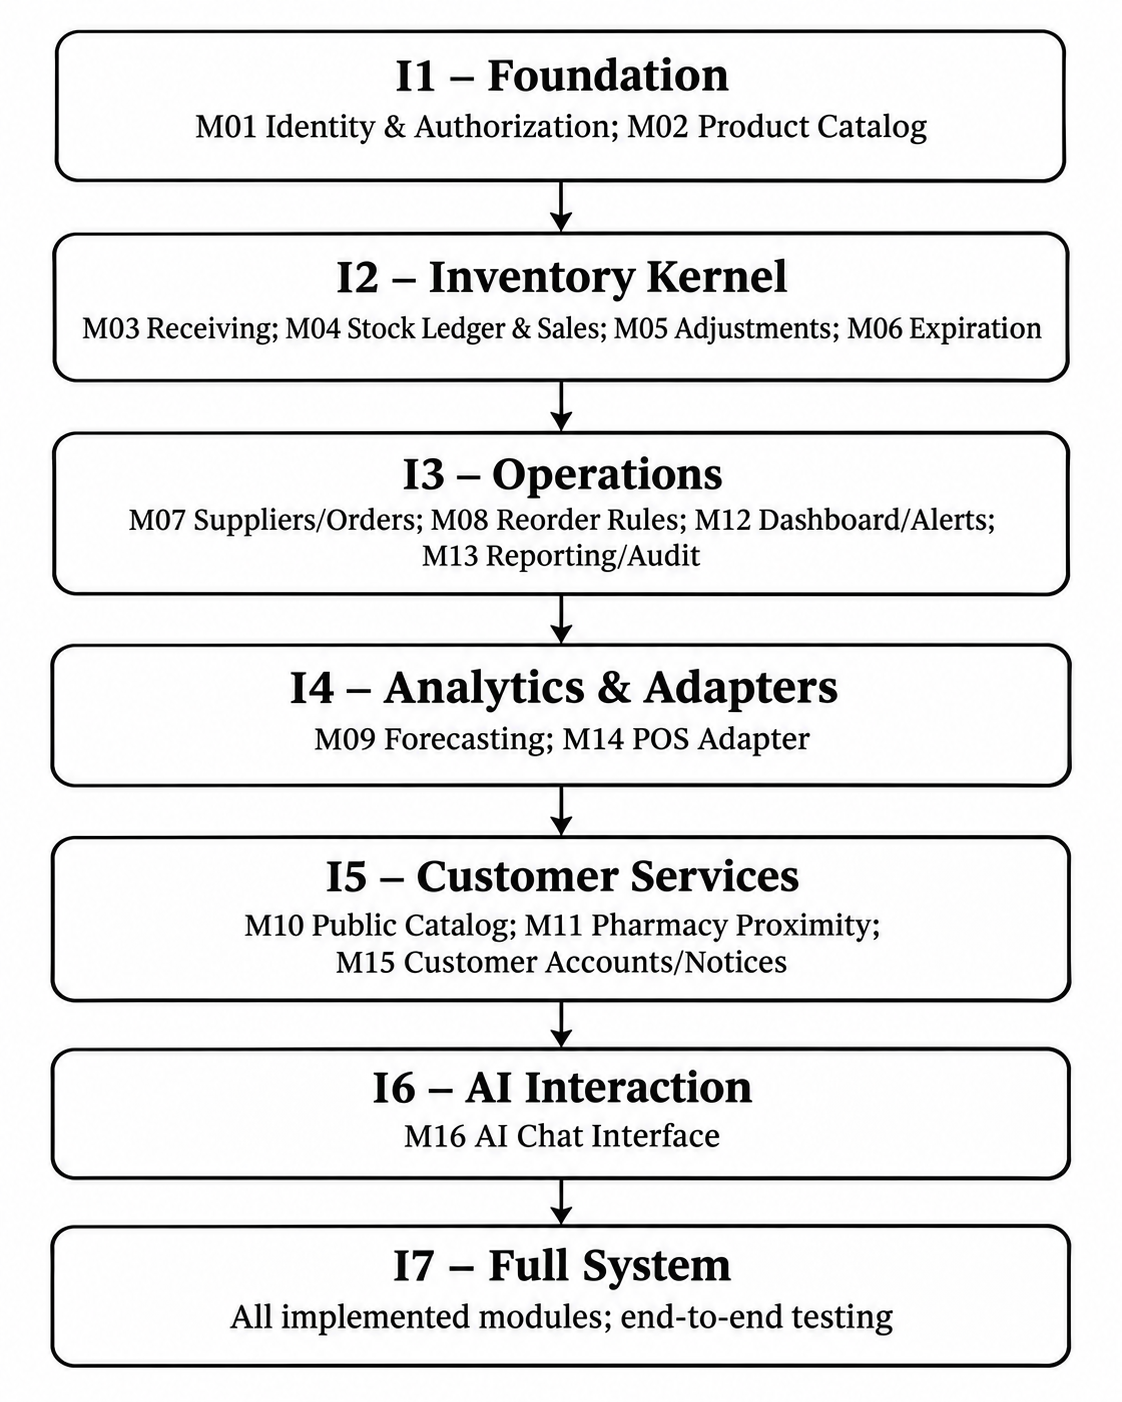
\includegraphics[width=3.40417in,height=4.25521in]{assets/test-plan/media/image1.png}

\emph{Figure 3.2.1. Dependency-driven integration sequence for the test plan}

{\def\LTcaptype{none} % do not increment counter
\begin{longtable}[]{|
  >{\raggedright\arraybackslash}m{(\linewidth - 6\tabcolsep - 4\arrayrulewidth) * \real{0.3333}}|
  >{\raggedright\arraybackslash}m{(\linewidth - 6\tabcolsep - 4\arrayrulewidth) * \real{0.3333}}|
  >{\raggedright\arraybackslash}m{(\linewidth - 6\tabcolsep - 4\arrayrulewidth) * \real{0.3333}}|}
\hline
\begin{minipage}[c]{\linewidth}\raggedright
\textbf{Increment}
\end{minipage} & \begin{minipage}[c]{\linewidth}\raggedright
\textbf{Modules introduced}
\end{minipage} & \begin{minipage}[c]{\linewidth}\raggedright
\textbf{Primary integration focus}
\end{minipage} \\
\hline
\endhead

\caption*{Table 3.2.1. Planned integration increments}\\
\endlastfoot
I1 - Foundation & M01 Identity and Authorization; M02 Product Catalog & Authentication context, RBAC, catalog validation, audit hooks. \\ \hline
I2 - Inventory kernel & M03 Receiving; M04 Stock Ledger and Sales; M05 Adjustments; M06 Expiration & Atomic stock changes, lot state, idempotency, approval, expiration blocking. \\ \hline
I3 - Operations & M07 Suppliers/Orders; M08 Reorder Rules; M12 Dashboard/Alerts; M13 Reporting/Audit & Order state transitions, threshold triggers, dashboards, audit/report consistency. \\ \hline
I4 - Analytics and POS & M09 Sales History/Forecasting; M14 POS Adapter & Historical ingestion, replay safety, forecast isolation, graceful dependency failure. \\ \hline
I5 - Customer services & M10 Public Catalog; M11 Pharmacy Proximity; M15 Customer Accounts/Notices & Safe public projection, distance sorting, privacy, optional notifications. \\ \hline
I6 - AI interaction & M16 AI Chat Interface & Advisory-only behavior, explanation, authorization boundary, no direct stock/order mutation. \\ \hline
I7 - Full system & All implemented modules & End-to-end functional, performance, reliability, security, and acceptance scenarios. \\ \hline
\end{longtable}
}

\subsection{3.3. Integration Interfaces to Exercise}\label{integration-interfaces-to-exercise}

\begin{itemize}
\item
  UI-to-API contracts and authorization context.
\item
  Application-service-to-repository/database transactions.
\item
  Stock Ledger calls from receiving, sales, adjustments, expiration/disposal, and POS ingestion.
\item
  Ordering state transitions and supplier adapter boundaries.
\item
  Sales-history-to-forecast data flow and read-only ML advisory boundary.
\item
  Public-search projection, location/proximity service, and customer account/notification flow.
\item
  Background worker interactions for alerts, forecasts, and notifications.
\end{itemize}

\clearpage
\section{4. Testing Methodologies and Technique Mapping}\label{testing-methodologies-and-technique-mapping}

\subsection{4.1. Required Techniques}\label{required-techniques}

The course requires walkthroughs, extensive logic testing, and input/output testing, with verification optionally applied where it is useful. The plan also includes automated unit tests, integration tests, functional black-box tests, performance evaluation, security checks, reliability/failure-injection tests, and acceptance testing. Each required technique is explicitly mapped to at least one module below.

{\def\LTcaptype{none} % do not increment counter
\begin{longtable}[]{|
  >{\raggedright\arraybackslash}m{(\linewidth - 6\tabcolsep - 4\arrayrulewidth) * \real{0.3333}}|
  >{\raggedright\arraybackslash}m{(\linewidth - 6\tabcolsep - 4\arrayrulewidth) * \real{0.3333}}|
  >{\raggedright\arraybackslash}m{(\linewidth - 6\tabcolsep - 4\arrayrulewidth) * \real{0.3333}}|}
\hline
\begin{minipage}[c]{\linewidth}\raggedright
\textbf{Technique}
\end{minipage} & \begin{minipage}[c]{\linewidth}\raggedright
\textbf{Primary module(s)}
\end{minipage} & \begin{minipage}[c]{\linewidth}\raggedright
\textbf{Planned application}
\end{minipage} \\
\hline
\endhead

\caption*{Table 4.1.1. Required testing-technique mapping}\\
\endlastfoot
Walkthrough & M04 Stock Ledger and Sales; M07 Suppliers and Purchase Orders & Peer-review transaction flow, state transitions, invariants, and failure handling before execution. \\ \hline
Logic testing & M04 Stock Ledger and Sales; M05 Adjustments; M06 Expiration & Exercise branches for sufficient/insufficient stock, concurrency, replay, approval states, and date boundaries. \\ \hline
Input/output testing & M02 Product Catalog; M03 Receiving; M10 Public Catalog & Boundary, malformed, missing, duplicate, and valid inputs with exact observable responses/error codes. \\ \hline
Verification & M04 Stock Ledger and Sales; M06 Expiration & Check invariants against pre/postconditions: nonnegative stock, exact-once deltas, expired-lot exclusion. \\ \hline
Performance evaluation & M10 Public Catalog; integrated backend & Measure search response and inventory-propagation targets under controlled load. \\ \hline
Acceptance testing & All implemented modules & Execute representative end-to-end pharmacist, technician, customer, and system workflows. \\ \hline
\end{longtable}
}

\subsection{4.2. Unit Testing Method}\label{unit-testing-method}

Each module will be tested in isolation through its public exports using mocked imports where necessary. Tests will cover normal behavior, boundary values, invalid inputs, authorization decisions, state transitions, and error codes. Database-facing modules will use a disposable test database or transaction rollback so each test begins from a known state. Time-sensitive modules will use a controllable clock to test expiration boundaries and scheduled behavior deterministically.

\subsection{4.3. Integration Testing Method}\label{integration-testing-method}

Integration tests will replace mocks incrementally with real project components in the sequence defined in Section 3. Tests will focus on contract mismatches, transaction boundaries, shared identifiers, error propagation, replay/idempotency, and authorization context. Each increment will preserve previously passing regression tests before the next module is added.

\subsection{4.4. Functional and Black-Box Testing}\label{functional-and-black-box-testing}

Functional tests will be written from the SRS rather than from implementation details. Inputs and expected user-visible outputs will be tested through the same public API or user interface path used by the final demonstration. Functional scenarios will include both successful actions and expected rejection behavior.

\subsection{4.5. Test Data and Environment}\label{test-data-and-environment}

All test data will be synthetic. The environment will contain multiple stores, staff roles, customers, active/inactive products, Schedule II and non-controlled products, lots with past/today/future expiration dates, suppliers, purchase orders, sales history, and repeated external event IDs. Tests must not depend on real patient or customer medical information. External services may be represented by deterministic mocks for failure and timeout cases.

\clearpage
\section{5. Detailed Planned Tests}\label{detailed-planned-tests}

The following planned test groups are intentionally representative rather than exhaustive. Each entry gives an objective, method, expected result, and success criterion. Individual automated cases may expand a group into several concrete test functions during implementation.

\subsection{5.01. TP-01 - M01 Identity and Authorization}\label{tp-01---m01-identity-and-authorization}

{\def\LTcaptype{none} % do not increment counter
\begin{longtable}[]{|
  >{\raggedright\arraybackslash}m{(\linewidth - 4\tabcolsep - 3\arrayrulewidth) * \real{0.5001}}|
  >{\raggedright\arraybackslash}m{(\linewidth - 4\tabcolsep - 3\arrayrulewidth) * \real{0.4999}}|}
\hline
\begin{minipage}[c]{\linewidth}\raggedright
\textbf{Item}
\end{minipage} & \begin{minipage}[c]{\linewidth}\raggedright
\textbf{Plan}
\end{minipage} \\
\hline
\endhead

\endlastfoot
Requirements & F1, F2 \\ \hline
Technique & Logic + I/O \\ \hline
Objective & Verify valid staff login, MFA completion, store-scoped RBAC, and denial of unauthorized actions. \\ \hline
Procedure / Expected Result & Valid credentials create the correct session; invalid/expired OTP is denied; a technician cannot perform manager-only approval; cross-store access is denied. \\ \hline
Success Criterion & All authorization decisions match the role/store policy and return the documented 401/403 behavior. \\ \hline
\end{longtable}
}

\subsection{5.02. TP-02 - M02 Product Catalog}\label{tp-02---m02-product-catalog}

{\def\LTcaptype{none} % do not increment counter
\begin{longtable}[]{|
  >{\raggedright\arraybackslash}m{(\linewidth - 4\tabcolsep - 3\arrayrulewidth) * \real{0.5001}}|
  >{\raggedright\arraybackslash}m{(\linewidth - 4\tabcolsep - 3\arrayrulewidth) * \real{0.4999}}|}
\hline
\begin{minipage}[c]{\linewidth}\raggedright
\textbf{Item}
\end{minipage} & \begin{minipage}[c]{\linewidth}\raggedright
\textbf{Plan}
\end{minipage} \\
\hline
\endhead

\endlastfoot
Requirements & F4, F19, F22 \\ \hline
Technique & I/O \\ \hline
Objective & Validate product create/update/deactivate behavior including NDC formatting and controlled-substance classification. \\ \hline
Procedure / Expected Result & Leading-zero NDC is preserved; duplicate NDC and missing required fields are rejected; deactivated product is omitted from normal listing. \\ \hline
Success Criterion & No malformed catalog record is committed and all valid records remain retrievable. \\ \hline
\end{longtable}
}

\subsection{5.03. TP-03 - M03 Stock Receiving}\label{tp-03---m03-stock-receiving}

{\def\LTcaptype{none} % do not increment counter
\begin{longtable}[]{|
  >{\raggedright\arraybackslash}m{(\linewidth - 4\tabcolsep - 3\arrayrulewidth) * \real{0.5001}}|
  >{\raggedright\arraybackslash}m{(\linewidth - 4\tabcolsep - 3\arrayrulewidth) * \real{0.4999}}|}
\hline
\begin{minipage}[c]{\linewidth}\raggedright
\textbf{Item}
\end{minipage} & \begin{minipage}[c]{\linewidth}\raggedright
\textbf{Plan}
\end{minipage} \\
\hline
\endhead

\endlastfoot
Requirements & F5, F7 \\ \hline
Technique & I/O + integration \\ \hline
Objective & Verify receipt of a new lot, matching existing lot, invalid quantity, inconsistent expiry, and replay of the same receipt. \\ \hline
Procedure / Expected Result & Valid receipt increases stock once and records movement/audit; zero quantity or inconsistent lot data is rejected; retry does not double-count. \\ \hline
Success Criterion & Stock delta equals accepted receipt quantity exactly once. \\ \hline
\end{longtable}
}

\subsection{5.04. TP-04 - M04 Stock Ledger and Sales}\label{tp-04---m04-stock-ledger-and-sales}

{\def\LTcaptype{none} % do not increment counter
\begin{longtable}[]{|
  >{\raggedright\arraybackslash}m{(\linewidth - 4\tabcolsep - 3\arrayrulewidth) * \real{0.5001}}|
  >{\raggedright\arraybackslash}m{(\linewidth - 4\tabcolsep - 3\arrayrulewidth) * \real{0.4999}}|}
\hline
\begin{minipage}[c]{\linewidth}\raggedright
\textbf{Item}
\end{minipage} & \begin{minipage}[c]{\linewidth}\raggedright
\textbf{Plan}
\end{minipage} \\
\hline
\endhead

\endlastfoot
Requirements & F3, F6, F7, F10 \\ \hline
Technique & Walkthrough + logic + verification \\ \hline
Objective & Verify exact-once sale decrement, lot selection, insufficient-stock rejection, and transaction atomicity. \\ \hline
Procedure / Expected Result & Valid sale decreases eligible lots; duplicate event replays without another decrement; insufficient stock returns error; failed transaction leaves all related data unchanged. \\ \hline
Success Criterion & No lot becomes negative; ledger and audit match the committed stock delta. \\ \hline
\end{longtable}
}

\subsection{5.05. TP-05 - M05 Adjustments and Cycle Counts}\label{tp-05---m05-adjustments-and-cycle-counts}

{\def\LTcaptype{none} % do not increment counter
\begin{longtable}[]{|
  >{\raggedright\arraybackslash}m{(\linewidth - 4\tabcolsep - 3\arrayrulewidth) * \real{0.5001}}|
  >{\raggedright\arraybackslash}m{(\linewidth - 4\tabcolsep - 3\arrayrulewidth) * \real{0.4999}}|}
\hline
\begin{minipage}[c]{\linewidth}\raggedright
\textbf{Item}
\end{minipage} & \begin{minipage}[c]{\linewidth}\raggedright
\textbf{Plan}
\end{minipage} \\
\hline
\endhead

\endlastfoot
Requirements & F6, F8 \\ \hline
Technique & Logic \\ \hline
Objective & Verify discrepancy creation, approval/rejection, stale-version handling, repeated approval, and role restriction. \\ \hline
Procedure / Expected Result & Request remains pending until authorized review; rejected request changes no stock; repeated approval cannot apply twice. \\ \hline
Success Criterion & Every approved adjustment is applied once, auditable, and cannot create negative stock. \\ \hline
\end{longtable}
}

\subsection{5.06. TP-06 - M06 Expiration Management}\label{tp-06---m06-expiration-management}

{\def\LTcaptype{none} % do not increment counter
\begin{longtable}[]{|
  >{\raggedright\arraybackslash}m{(\linewidth - 4\tabcolsep - 3\arrayrulewidth) * \real{0.5001}}|
  >{\raggedright\arraybackslash}m{(\linewidth - 4\tabcolsep - 3\arrayrulewidth) * \real{0.4999}}|}
\hline
\begin{minipage}[c]{\linewidth}\raggedright
\textbf{Item}
\end{minipage} & \begin{minipage}[c]{\linewidth}\raggedright
\textbf{Plan}
\end{minipage} \\
\hline
\endhead

\endlastfoot
Requirements & F9-F11 \\ \hline
Technique & Logic + verification \\ \hline
Objective & Verify expired/soon-to-expire classification, midnight boundary, alert deduplication, and sale exclusion. \\ \hline
Procedure / Expected Result & Past date is expired; today/future thresholds classify correctly; rerun does not duplicate daily alert; expired lot is unsellable. \\ \hline
Success Criterion & Classification matches the store-local calendar and expired inventory never contributes to sellable quantity. \\ \hline
\end{longtable}
}

\subsection{5.07. TP-07 - M07 Suppliers and Purchase Orders}\label{tp-07---m07-suppliers-and-purchase-orders}

{\def\LTcaptype{none} % do not increment counter
\begin{longtable}[]{|
  >{\raggedright\arraybackslash}m{(\linewidth - 4\tabcolsep - 3\arrayrulewidth) * \real{0.5001}}|
  >{\raggedright\arraybackslash}m{(\linewidth - 4\tabcolsep - 3\arrayrulewidth) * \real{0.4999}}|}
\hline
\begin{minipage}[c]{\linewidth}\raggedright
\textbf{Item}
\end{minipage} & \begin{minipage}[c]{\linewidth}\raggedright
\textbf{Plan}
\end{minipage} \\
\hline
\endhead

\endlastfoot
Requirements & F12-F14 \\ \hline
Technique & Walkthrough + logic \\ \hline
Objective & Verify draft creation, manager approval, send eligibility, retry, and status transitions. \\ \hline
Procedure / Expected Result & Only approved order can be sent; technician approval fails; failed adapter call can be retried without duplicate order state. \\ \hline
Success Criterion & State machine never skips required approval and every transition is audited. \\ \hline
\end{longtable}
}

\subsection{5.08. TP-08 - M08 Reorder Rules and Suggestions}\label{tp-08---m08-reorder-rules-and-suggestions}

{\def\LTcaptype{none} % do not increment counter
\begin{longtable}[]{|
  >{\raggedright\arraybackslash}m{(\linewidth - 4\tabcolsep - 3\arrayrulewidth) * \real{0.5001}}|
  >{\raggedright\arraybackslash}m{(\linewidth - 4\tabcolsep - 3\arrayrulewidth) * \real{0.4999}}|}
\hline
\begin{minipage}[c]{\linewidth}\raggedright
\textbf{Item}
\end{minipage} & \begin{minipage}[c]{\linewidth}\raggedright
\textbf{Plan}
\end{minipage} \\
\hline
\endhead

\endlastfoot
Requirements & F13, F17, F18 \\ \hline
Technique & Logic \\ \hline
Objective & Verify threshold trigger and advisory recommendation workflow. \\ \hline
Procedure / Expected Result & At/below reorder point creates alert/draft suggestion; above threshold does not; AI/rule suggestion cannot directly place an order. \\ \hline
Success Criterion & Every order-impacting action requires authorized human approval. \\ \hline
\end{longtable}
}

\subsection{5.09. TP-09 - M09 Sales History and Forecasting}\label{tp-09---m09-sales-history-and-forecasting}

{\def\LTcaptype{none} % do not increment counter
\begin{longtable}[]{|
  >{\raggedright\arraybackslash}m{(\linewidth - 4\tabcolsep - 3\arrayrulewidth) * \real{0.5001}}|
  >{\raggedright\arraybackslash}m{(\linewidth - 4\tabcolsep - 3\arrayrulewidth) * \real{0.4999}}|}
\hline
\begin{minipage}[c]{\linewidth}\raggedright
\textbf{Item}
\end{minipage} & \begin{minipage}[c]{\linewidth}\raggedright
\textbf{Plan}
\end{minipage} \\
\hline
\endhead

\endlastfoot
Requirements & F16, F17 \\ \hline
Technique & I/O + reliability \\ \hline
Objective & Verify 7/30/90-day forecast interface, data sufficiency handling, and model-unavailable fallback. \\ \hline
Procedure / Expected Result & Valid history returns advisory forecast object; unsupported horizon is rejected; model outage leaves inventory kernel usable. \\ \hline
Success Criterion & Forecast generation never mutates inventory or purchase-order state. \\ \hline
\end{longtable}
}

\subsection{5.10. TP-10 - M10 Public Catalog and Availability}\label{tp-10---m10-public-catalog-and-availability}

{\def\LTcaptype{none} % do not increment counter
\begin{longtable}[]{|
  >{\raggedright\arraybackslash}m{(\linewidth - 4\tabcolsep - 3\arrayrulewidth) * \real{0.5001}}|
  >{\raggedright\arraybackslash}m{(\linewidth - 4\tabcolsep - 3\arrayrulewidth) * \real{0.4999}}|}
\hline
\begin{minipage}[c]{\linewidth}\raggedright
\textbf{Item}
\end{minipage} & \begin{minipage}[c]{\linewidth}\raggedright
\textbf{Plan}
\end{minipage} \\
\hline
\endhead

\endlastfoot
Requirements & F19, F20, F22 \\ \hline
Technique & I/O + security \\ \hline
Objective & Verify search by brand/generic/NDC, coarse availability, cash price, and Schedule II masking. \\ \hline
Procedure / Expected Result & Public result shows In Stock/Low Stock/Out of Stock but never exact count; Schedule II shows contact-pharmacy message. \\ \hline
Success Criterion & No private lot quantity or restricted availability is exposed. \\ \hline
\end{longtable}
}

\subsection{5.11. TP-11 - M11 Pharmacy Proximity}\label{tp-11---m11-pharmacy-proximity}

{\def\LTcaptype{none} % do not increment counter
\begin{longtable}[]{|
  >{\raggedright\arraybackslash}m{(\linewidth - 4\tabcolsep - 3\arrayrulewidth) * \real{0.5001}}|
  >{\raggedright\arraybackslash}m{(\linewidth - 4\tabcolsep - 3\arrayrulewidth) * \real{0.4999}}|}
\hline
\begin{minipage}[c]{\linewidth}\raggedright
\textbf{Item}
\end{minipage} & \begin{minipage}[c]{\linewidth}\raggedright
\textbf{Plan}
\end{minipage} \\
\hline
\endhead

\endlastfoot
Requirements & F21 \\ \hline
Technique & Functional + I/O \\ \hline
Objective & Verify ZIP/device-location input, distance ordering, consent handling, and the required nearby-pharmacy list without an embedded map. Embedded map integration may be deferred. \\ \hline
Procedure / Expected Result & Stores are sorted nearest-first; location use requires consent; entered/device location is not persisted; dependency failure is explicit. \\ \hline
Success Criterion & Correct ordering for controlled coordinates and no stored customer location. \\ \hline
\end{longtable}
}

\subsection{5.12. TP-12 - M12 Dashboard and Alerts}\label{tp-12---m12-dashboard-and-alerts}

{\def\LTcaptype{none} % do not increment counter
\begin{longtable}[]{|
  >{\raggedright\arraybackslash}m{(\linewidth - 4\tabcolsep - 3\arrayrulewidth) * \real{0.5001}}|
  >{\raggedright\arraybackslash}m{(\linewidth - 4\tabcolsep - 3\arrayrulewidth) * \real{0.4999}}|}
\hline
\begin{minipage}[c]{\linewidth}\raggedright
\textbf{Item}
\end{minipage} & \begin{minipage}[c]{\linewidth}\raggedright
\textbf{Plan}
\end{minipage} \\
\hline
\endhead

\endlastfoot
Requirements & F9, F10, F13, F24 \\ \hline
Technique & Integration \\ \hline
Objective & Verify dashboard aggregation from low-stock, expiration, pending order, and AI alert sources. \\ \hline
Procedure / Expected Result & Dashboard counts/items match underlying test data and refresh after source changes. \\ \hline
Success Criterion & The displayed summary agrees with source records within the defined update window. \\ \hline
\end{longtable}
}

\subsection{5.13. TP-13 - M13 Reporting and Audit}\label{tp-13---m13-reporting-and-audit}

{\def\LTcaptype{none} % do not increment counter
\begin{longtable}[]{|
  >{\raggedright\arraybackslash}m{(\linewidth - 4\tabcolsep - 3\arrayrulewidth) * \real{0.5001}}|
  >{\raggedright\arraybackslash}m{(\linewidth - 4\tabcolsep - 3\arrayrulewidth) * \real{0.4999}}|}
\hline
\begin{minipage}[c]{\linewidth}\raggedright
\textbf{Item}
\end{minipage} & \begin{minipage}[c]{\linewidth}\raggedright
\textbf{Plan}
\end{minipage} \\
\hline
\endhead

\endlastfoot
Requirements & F3, F25 \\ \hline
Technique & Functional + verification \\ \hline
Objective & Verify audit completeness and report calculations/exports. \\ \hline
Procedure / Expected Result & Inventory changes appear with actor/time/action; reports reconcile with seeded movements and expiration loss data. \\ \hline
Success Criterion & No committed inventory mutation lacks an audit record; report totals reconcile to source rows. \\ \hline
\end{longtable}
}

\subsection{5.14. TP-14 - M14 POS Integration Adapter}\label{tp-14---m14-pos-integration-adapter}

{\def\LTcaptype{none} % do not increment counter
\begin{longtable}[]{|
  >{\raggedright\arraybackslash}m{(\linewidth - 4\tabcolsep - 3\arrayrulewidth) * \real{0.5001}}|
  >{\raggedright\arraybackslash}m{(\linewidth - 4\tabcolsep - 3\arrayrulewidth) * \real{0.4999}}|}
\hline
\begin{minipage}[c]{\linewidth}\raggedright
\textbf{Item}
\end{minipage} & \begin{minipage}[c]{\linewidth}\raggedright
\textbf{Plan}
\end{minipage} \\
\hline
\endhead

\endlastfoot
Requirements & F6, F10 \\ \hline
Technique & Integration + failure injection \\ \hline
Objective & Verify normal sale ingestion, duplicate event, temporary outage, retry, and invalid payload. \\ \hline
Procedure / Expected Result & Valid POS event applies once; duplicate ID does not double-decrement; retry retains same event identity; malformed payload is rejected. \\ \hline
Success Criterion & At-least-once delivery produces exactly-once inventory effect. \\ \hline
\end{longtable}
}

\subsection{5.15. TP-15 - M15 Customer Accounts and Notices}\label{tp-15---m15-customer-accounts-and-notices}

{\def\LTcaptype{none} % do not increment counter
\begin{longtable}[]{|
  >{\raggedright\arraybackslash}m{(\linewidth - 4\tabcolsep - 3\arrayrulewidth) * \real{0.5001}}|
  >{\raggedright\arraybackslash}m{(\linewidth - 4\tabcolsep - 3\arrayrulewidth) * \real{0.4999}}|}
\hline
\begin{minipage}[c]{\linewidth}\raggedright
\textbf{Item}
\end{minipage} & \begin{minipage}[c]{\linewidth}\raggedright
\textbf{Plan}
\end{minipage} \\
\hline
\endhead

\endlastfoot
Requirements & F2, F23 \\ \hline
Technique & I/O + privacy \\ \hline
Objective & Verify optional registration, subscription, back-in-stock notice, and account-independent search. \\ \hline
Procedure / Expected Result & Unregistered search works; registered customer may subscribe; notice fires on qualifying transition without exposing inventory count. \\ \hline
Success Criterion & Subscription behavior adds no requirement for an account to perform public search. \\ \hline
\end{longtable}
}

\subsection{5.16. TP-16 - M16 AI Chat Interface}\label{tp-16---m16-ai-chat-interface}

{\def\LTcaptype{none} % do not increment counter
\begin{longtable}[]{|
  >{\raggedright\arraybackslash}m{(\linewidth - 4\tabcolsep - 3\arrayrulewidth) * \real{0.5001}}|
  >{\raggedright\arraybackslash}m{(\linewidth - 4\tabcolsep - 3\arrayrulewidth) * \real{0.4999}}|}
\hline
\begin{minipage}[c]{\linewidth}\raggedright
\textbf{Item}
\end{minipage} & \begin{minipage}[c]{\linewidth}\raggedright
\textbf{Plan}
\end{minipage} \\
\hline
\endhead

\endlastfoot
Requirements & F15, F18 \\ \hline
Technique & Functional + security \\ \hline
Objective & Verify advisory answers, explanation, unsupported medical request handling, and mutation boundary. \\ \hline
Procedure / Expected Result & Chat may summarize inventory recommendations but cannot directly modify stock or place order; medical/dosing advice is not provided. \\ \hline
Success Criterion & All state-changing requests are refused or routed to authorized application workflow. \\ \hline
\end{longtable}
}

\subsection{5.17. TP-17 - End-to-end Receive-to-Sale}\label{tp-17---end-to-end-receive-to-sale}

{\def\LTcaptype{none} % do not increment counter
\begin{longtable}[]{|
  >{\raggedright\arraybackslash}m{(\linewidth - 4\tabcolsep - 3\arrayrulewidth) * \real{0.5001}}|
  >{\raggedright\arraybackslash}m{(\linewidth - 4\tabcolsep - 3\arrayrulewidth) * \real{0.4999}}|}
\hline
\begin{minipage}[c]{\linewidth}\raggedright
\textbf{Item}
\end{minipage} & \begin{minipage}[c]{\linewidth}\raggedright
\textbf{Plan}
\end{minipage} \\
\hline
\endhead

\endlastfoot
Requirements & F3-F7, F9-F10 \\ \hline
Technique & Functional \\ \hline
Objective & Receive a valid lot, observe stock, process sale, and inspect resulting ledger/audit/expiration state. \\ \hline
Procedure / Expected Result & Receipt increases stock; sale decreases it; visible stock reflects result; audit and movement history remain consistent. \\ \hline
Success Criterion & End-to-end quantity equation balances and all records are traceable. \\ \hline
\end{longtable}
}

\subsection{5.18. TP-18 - End-to-end Reorder Approval}\label{tp-18---end-to-end-reorder-approval}

{\def\LTcaptype{none} % do not increment counter
\begin{longtable}[]{|
  >{\raggedright\arraybackslash}m{(\linewidth - 4\tabcolsep - 3\arrayrulewidth) * \real{0.5001}}|
  >{\raggedright\arraybackslash}m{(\linewidth - 4\tabcolsep - 3\arrayrulewidth) * \real{0.4999}}|}
\hline
\begin{minipage}[c]{\linewidth}\raggedright
\textbf{Item}
\end{minipage} & \begin{minipage}[c]{\linewidth}\raggedright
\textbf{Plan}
\end{minipage} \\
\hline
\endhead

\endlastfoot
Requirements & F12-F18, F24 \\ \hline
Technique & Functional \\ \hline
Objective & Drive stock to threshold, create recommendation/draft order, obtain manager approval, and send through adapter mock. \\ \hline
Procedure / Expected Result & Alert and draft appear, human approval changes state, then send occurs; AI output alone does not send. \\ \hline
Success Criterion & No purchase order leaves Draft without authorized approval. \\ \hline
\end{longtable}
}

\subsection{5.19. TP-19 - Customer Search Journey}\label{tp-19---customer-search-journey}

{\def\LTcaptype{none} % do not increment counter
\begin{longtable}[]{|
  >{\raggedright\arraybackslash}m{(\linewidth - 4\tabcolsep - 3\arrayrulewidth) * \real{0.5001}}|
  >{\raggedright\arraybackslash}m{(\linewidth - 4\tabcolsep - 3\arrayrulewidth) * \real{0.4999}}|}
\hline
\begin{minipage}[c]{\linewidth}\raggedright
\textbf{Item}
\end{minipage} & \begin{minipage}[c]{\linewidth}\raggedright
\textbf{Plan}
\end{minipage} \\
\hline
\endhead

\endlastfoot
Requirements & F19-F23 \\ \hline
Technique & Functional \\ \hline
Objective & Search product, view price/coarse availability, locate nearest pharmacy, and subscribe when out of stock. \\ \hline
Procedure / Expected Result & Customer obtains safe availability and price, nearest store ordering, and optional notice workflow. \\ \hline
Success Criterion & All public privacy rules and expected outputs hold across the complete journey. \\ \hline
\end{longtable}
}

\subsection{5.20. TP-20 - Concurrent / Replay Inventory Stress}\label{tp-20---concurrent-replay-inventory-stress}

{\def\LTcaptype{none} % do not increment counter
\begin{longtable}[]{|
  >{\raggedright\arraybackslash}m{(\linewidth - 4\tabcolsep - 3\arrayrulewidth) * \real{0.5001}}|
  >{\raggedright\arraybackslash}m{(\linewidth - 4\tabcolsep - 3\arrayrulewidth) * \real{0.4999}}|}
\hline
\begin{minipage}[c]{\linewidth}\raggedright
\textbf{Item}
\end{minipage} & \begin{minipage}[c]{\linewidth}\raggedright
\textbf{Plan}
\end{minipage} \\
\hline
\endhead

\endlastfoot
Requirements & F3, F6, F7 \\ \hline
Technique & Logic + performance \\ \hline
Objective & Submit concurrent sales and replayed event IDs against limited stock. \\ \hline
Procedure / Expected Result & Only available units are committed, excess request is rejected, replay does not double-apply, and final quantity is nonnegative. \\ \hline
Success Criterion & Final stock and ledger equal the serializable expected result with no duplicate movement for one event ID. \\ \hline
\end{longtable}
}

\clearpage
\section{6. Non-Functional Evaluation}\label{non-functional-evaluation}

\subsection{6.1. Performance and Scalability}\label{performance-and-scalability}

{\def\LTcaptype{none} % do not increment counter
\begin{longtable}[]{|
  >{\raggedright\arraybackslash}m{(\linewidth - 6\tabcolsep - 4\arrayrulewidth) * \real{0.3333}}|
  >{\raggedright\arraybackslash}m{(\linewidth - 6\tabcolsep - 4\arrayrulewidth) * \real{0.3333}}|
  >{\raggedright\arraybackslash}m{(\linewidth - 6\tabcolsep - 4\arrayrulewidth) * \real{0.3333}}|}
\hline
\begin{minipage}[c]{\linewidth}\raggedright
\textbf{Metric}
\end{minipage} & \begin{minipage}[c]{\linewidth}\raggedright
\textbf{Method}
\end{minipage} & \begin{minipage}[c]{\linewidth}\raggedright
\textbf{Success target}
\end{minipage} \\
\hline
\endhead

\caption*{Table 6.1.1. Performance evaluation plan}\\
\endlastfoot
Customer search response & Run repeated representative brand/generic/NDC searches while recording server and client elapsed time under controlled concurrent load. & \textless=2 seconds for the target test configuration. \\ \hline
Inventory propagation & Commit receipt/sale/adjustment and poll staff views until new value is visible. & \textless=5 seconds. \\ \hline
Concurrent customer sessions & Use load tools or scripted clients against read endpoints with synthetic catalog data. & System remains responsive and error rate stays within agreed project threshold; scalability result recorded even if full 1,000-session target cannot be reproduced on course hardware. \\ \hline
Catalog scale & Seed representative high-volume product/store records and repeat search/filter/report operations. & No correctness failure; measured performance documented against SRS target. \\ \hline
\end{longtable}
}

\subsection{6.2. Reliability and Recovery}\label{reliability-and-recovery}

Reliability tests will deliberately interrupt or fail POS, supplier, forecast, map, and notification dependencies. The expected behavior is an explicit recoverable error, queued/retried work where the design defines it, and no corruption of committed inventory. Database backup and recovery procedures will be exercised if implemented for the prototype; the recovery evidence will state the measured result rather than assuming the four-hour SRS objective was achieved.

\subsection{6.3. Security and Privacy}\label{security-and-privacy}

\begin{itemize}
\item
  Authentication and MFA failure paths.
\item
  Role- and store-scope authorization on every state-changing operation.
\item
  Schedule II public availability masking.
\item
  No exact public stock quantities.
\item
  No persistence of customer device location or entered ZIP beyond what the implementation requires for the current request.
\item
  Input validation against malformed identifiers, unexpected payloads, and common web injection patterns appropriate to the selected stack.
\item
  Audit trail integrity for inventory changes and approvals.
\end{itemize}

\subsection{6.4. Usability and Accessibility}\label{usability-and-accessibility}

The team will perform a task walkthrough of common pharmacist, technician, and customer workflows, checking that the dashboard provides a direct path to common tasks and that interface labels/error messages are understandable. Where a web interface is implemented, accessibility checks will cover keyboard navigation, form labels, semantic structure, contrast, and other WCAG 2.1 AA-relevant items that can be evaluated within the prototype.

\subsection{6.5. Machine-Learning Quality}\label{machine-learning-quality}

For products with at least six months of synthetic or prepared sales history, forecast output will be compared with held-out known values and MAPE will be recorded for 7-, 30-, and 90-day horizons. The SRS target is MAPE of 20\% or less. If the available project data are insufficient for a meaningful statistical claim, the test report will document the limitation and will still verify interface correctness, horizon handling, deterministic preprocessing, and the advisory-only safety boundary.

\clearpage
\section{7. Responsibilities and Master Schedule}\label{responsibilities-and-master-schedule}

\subsection{7.1. Proposed Ownership}\label{proposed-ownership}

Because the Week 8 design document leaves individual module ownership unconfirmed, the assignments below are a balanced proposal for the test-planning draft, not a statement of prior team agreement. The team should confirm or edit ownership before the Week 11 final test plan.

{\def\LTcaptype{none} % do not increment counter
\begin{longtable}[]{|
  >{\raggedright\arraybackslash}m{(\linewidth - 6\tabcolsep - 4\arrayrulewidth) * \real{0.3333}}|
  >{\raggedright\arraybackslash}m{(\linewidth - 6\tabcolsep - 4\arrayrulewidth) * \real{0.3333}}|
  >{\raggedright\arraybackslash}m{(\linewidth - 6\tabcolsep - 4\arrayrulewidth) * \real{0.3333}}|}
\hline
\begin{minipage}[c]{\linewidth}\raggedright
\textbf{Team member}
\end{minipage} & \begin{minipage}[c]{\linewidth}\raggedright
\textbf{Proposed primary test responsibility}
\end{minipage} & \begin{minipage}[c]{\linewidth}\raggedright
\textbf{Cross-review responsibility}
\end{minipage} \\
\hline
\endhead

\caption*{Table 7.1.1. Proposed team test responsibilities}\\
\endlastfoot
Maria Molano Escobar & M01-M04; foundation and inventory-kernel unit/integration tests & Review customer/public test cases. \\ \hline
Marko Maksuti & M05-M08; adjustment, expiration, ordering, reorder logic & Review POS/concurrency and performance cases. \\ \hline
Ryan Petillo & M09-M12; forecast, public search, proximity, dashboard & Review inventory-kernel and authorization cases. \\ \hline
Samuel Cordova & M13-M16; reporting, POS adapter, customer notices, AI chat & Review ordering/forecast and acceptance cases. \\ \hline
All team members & End-to-end functional, regression, performance/reliability, acceptance demonstration & Peer walkthroughs and defect triage. \\ \hline
\end{longtable}
}

\subsection{7.2. Master Test Schedule}\label{master-test-schedule}

{\def\LTcaptype{none} % do not increment counter
\begin{longtable}[]{|
  >{\raggedright\arraybackslash}m{(\linewidth - 6\tabcolsep - 4\arrayrulewidth) * \real{0.3333}}|
  >{\raggedright\arraybackslash}m{(\linewidth - 6\tabcolsep - 4\arrayrulewidth) * \real{0.3333}}|
  >{\raggedright\arraybackslash}m{(\linewidth - 6\tabcolsep - 4\arrayrulewidth) * \real{0.3333}}|}
\hline
\begin{minipage}[c]{\linewidth}\raggedright
\textbf{Date / milestone}
\end{minipage} & \begin{minipage}[c]{\linewidth}\raggedright
\textbf{Planned activity}
\end{minipage} & \begin{minipage}[c]{\linewidth}\raggedright
\textbf{Responsible}
\end{minipage} \\
\hline
\endhead

\caption*{Table 7.2.1. Master test plan schedule}\\
\endlastfoot
Nov 12, 2026 - Week 10 & Submit initial test plan; confirm test architecture, technique mapping, and proposed ownership. & All; document editor/team \\ \hline
Nov 13-15 & Prepare unit-test harnesses, synthetic fixtures, mocks/stubs; execute walkthroughs for M04 and M07. & Module test owners + peer reviewer \\ \hline
Nov 16-18 & Execute critical unit tests and Integration I1-I3; log defects; begin regression suite. & Owners of M01-M08, M12-M13 \\ \hline
Nov 19, 2026 - Week 11 & Submit Final Test Plan; top-level code for main modules due. & All \\ \hline
Nov 20-24 & Integration I4-I6; POS/forecast/customer/AI tests; first performance baseline. & Owners of M09-M16 \\ \hline
Nov 25 & Proposed individual test-report checkpoint: each member submits/merges a brief report for at least one executed test set. & Each team member \\ \hline
Nov 26-Dec 1 & Full-system functional regression, security/privacy checks, performance/reliability retests; defect correction. & All \\ \hline
Dec 2 & Acceptance-candidate build freeze; reset demonstration data; final acceptance rehearsal. & All \\ \hline
Dec 3, 2026 - Week 13 & User Manual Draft due / final exam; preserve stable test baseline. & All \\ \hline
Dec 4-9 & Final regression on accepted fixes; package test evidence and demo checklist. & All \\ \hline
Dec 10, 2026 - Week 14 & Demo/presentation and final project submission (subject to course change). & All \\ \hline
\end{longtable}
}

\subsection{7.3. Individual Test Report Contents}\label{individual-test-report-contents}

Each individual test report should identify the test set, module/build tested, author/tester, date, environment, input data, steps, expected result, observed result, pass/fail status, defects raised, and retest outcome. Screenshots or logs should be included only where they add evidence; raw sensitive or real customer data must not be used.

\clearpage
\section{8. Monitoring, Reporting, and Correcting Procedures}\label{monitoring-reporting-and-correcting-procedures}

\subsection{8.1. Test Monitoring}\label{test-monitoring}

The team will maintain one shared test-status record with each planned test marked Not Ready, Ready, Running, Pass, Fail, Blocked, or Deferred. At each team review, the assigned coordinator/editor will compare the record with the master schedule, identify missing evidence or late tests, and report blockers to the full team. A test may be marked Pass only when its expected result and success criterion are both satisfied on the identified build.

\subsection{8.2. Defect Reporting}\label{defect-reporting}

{\def\LTcaptype{none} % do not increment counter
\begin{longtable}[]{|
  >{\raggedright\arraybackslash}m{(\linewidth - 4\tabcolsep - 3\arrayrulewidth) * \real{0.5001}}|
  >{\raggedright\arraybackslash}m{(\linewidth - 4\tabcolsep - 3\arrayrulewidth) * \real{0.4999}}|}
\hline
\begin{minipage}[c]{\linewidth}\raggedright
\textbf{Field}
\end{minipage} & \begin{minipage}[c]{\linewidth}\raggedright
\textbf{Required content}
\end{minipage} \\
\hline
\endhead

\caption*{Table 8.2.1. Required defect-report fields}\\
\endlastfoot
Defect ID & Unique identifier, e.g., BUG-017. \\ \hline
Summary & Short statement of the observed problem. \\ \hline
Build / environment & Commit/build identifier and relevant configuration. \\ \hline
Preconditions / data & State required to reproduce the problem. \\ \hline
Steps to reproduce & Minimal ordered sequence. \\ \hline
Expected result & Behavior required by SRS/design/test oracle. \\ \hline
Observed result & Actual behavior, error, log, or screenshot reference. \\ \hline
Severity / priority & Severity based on impact; priority based on repair urgency. \\ \hline
Owner / status & Assigned developer and Open/In Progress/Fixed/Retest/Closed. \\ \hline
Traceability & Related test ID, module ID, and requirement ID. \\ \hline
\end{longtable}
}

\subsection{8.3. Severity Definitions}\label{severity-definitions}

{\def\LTcaptype{none} % do not increment counter
\begin{longtable}[]{|
  >{\raggedright\arraybackslash}m{(\linewidth - 4\tabcolsep - 3\arrayrulewidth) * \real{0.5001}}|
  >{\raggedright\arraybackslash}m{(\linewidth - 4\tabcolsep - 3\arrayrulewidth) * \real{0.4999}}|}
\hline
\begin{minipage}[c]{\linewidth}\raggedright
\textbf{Severity}
\end{minipage} & \begin{minipage}[c]{\linewidth}\raggedright
\textbf{Definition}
\end{minipage} \\
\hline
\endhead

\caption*{Table 8.3.1. Defect severity levels}\\
\endlastfoot
S1 - Critical & Data corruption, security/privacy breach, negative inventory, unauthorized approval, expired-stock sale, or system unusable for acceptance path. \\ \hline
S2 - Major & Required function incorrect or unavailable with no reasonable workaround. \\ \hline
S3 - Moderate & Incorrect secondary behavior or requirement with workaround; does not corrupt protected state. \\ \hline
S4 - Minor & Cosmetic, wording, low-impact usability, or documentation issue. \\ \hline
\end{longtable}
}

\subsection{8.4. Correction, Retest, and Regression}\label{correction-retest-and-regression}

A developer fixes the defect on a traceable change. The original tester or a peer then reruns the failing case on the corrected build and records the retest result. Any change to shared inventory, authorization, API contracts, database schema, state machines, or external adapters triggers the relevant regression subset. Severity 1 defects require full-system regression of the affected workflow before acceptance. A defect is closed only after a successful retest or an explicitly documented disposition agreed by the team.

\subsection{8.5. Change Control for the Test Plan}\label{change-control-for-the-test-plan}

When a requirement, interface, or design decision changes, the team updates the affected test cases and traceability entries in the same revision. New behavior is not treated as tested merely because an older test still passes. The revision history will identify material changes between the Week 10 initial draft and Week 11 final plan.

\clearpage
\section{9. Traceability}\label{traceability}

\subsection{9.1. Requirement-to-Test Coverage}\label{requirement-to-test-coverage}

{\def\LTcaptype{none} % do not increment counter
\begin{longtable}[]{|
  >{\raggedright\arraybackslash}m{(\linewidth - 6\tabcolsep - 4\arrayrulewidth) * \real{0.3333}}|
  >{\raggedright\arraybackslash}m{(\linewidth - 6\tabcolsep - 4\arrayrulewidth) * \real{0.3333}}|
  >{\raggedright\arraybackslash}m{(\linewidth - 6\tabcolsep - 4\arrayrulewidth) * \real{0.3333}}|}
\hline
\begin{minipage}[c]{\linewidth}\raggedright
\textbf{Requirement group}
\end{minipage} & \begin{minipage}[c]{\linewidth}\raggedright
\textbf{Functions}
\end{minipage} & \begin{minipage}[c]{\linewidth}\raggedright
\textbf{Primary planned tests}
\end{minipage} \\
\hline
\endhead

\caption*{Table 9.1.1. Functional requirement traceability summary}\\
\endlastfoot
User management / security & F1-F3 & TP-01, TP-13, TP-17 \\ \hline
Inventory management & F4-F8 & TP-02 through TP-05, TP-14, TP-17, TP-20 \\ \hline
Expiration management & F9-F11 & TP-06, TP-12, TP-17 \\ \hline
Reordering / suppliers & F12-F15 & TP-07, TP-08, TP-18 \\ \hline
ML analytics / approval & F16-F18 & TP-08, TP-09, TP-16, TP-18 \\ \hline
Customer information portal & F19-F23 & TP-10, TP-11, TP-15, TP-19 \\ \hline
Dashboard / reporting & F24-F25 & TP-12, TP-13, TP-18 \\ \hline
\end{longtable}
}

\subsection{9.2. Module-to-Test Coverage}\label{module-to-test-coverage}

{\def\LTcaptype{none} % do not increment counter
\begin{longtable}[]{|
  >{\raggedright\arraybackslash}m{(\linewidth - 4\tabcolsep - 3\arrayrulewidth) * \real{0.5001}}|
  >{\raggedright\arraybackslash}m{(\linewidth - 4\tabcolsep - 3\arrayrulewidth) * \real{0.4999}}|}
\hline
\begin{minipage}[c]{\linewidth}\raggedright
\textbf{Module}
\end{minipage} & \begin{minipage}[c]{\linewidth}\raggedright
\textbf{Primary planned test}
\end{minipage} \\
\hline
\endhead

\caption*{Table 9.2.1. Module-to-test coverage}\\
\endlastfoot
M01 Identity and Authorization & TP-01 \\ \hline
M02 Product Catalog & TP-02 \\ \hline
M03 Stock Receiving and Lot Registry & TP-03 \\ \hline
M04 Stock Ledger and Sales & TP-04, TP-17, TP-20 \\ \hline
M05 Adjustments and Cycle Counts & TP-05 \\ \hline
M06 Expiration Management & TP-06 \\ \hline
M07 Suppliers and Purchase Orders & TP-07, TP-18 \\ \hline
M08 Reorder Rules and Suggestions & TP-08, TP-18 \\ \hline
M09 Sales History and Forecasting & TP-09 \\ \hline
M10 Public Catalog and Availability & TP-10, TP-19 \\ \hline
M11 Pharmacy Proximity & TP-11, TP-19 \\ \hline
M12 Dashboard and Alerts & TP-12, TP-18 \\ \hline
M13 Reporting and Audit & TP-13, TP-17 \\ \hline
M14 POS Integration Adapter & TP-14, TP-20 \\ \hline
M15 Customer Accounts and Notices & TP-15, TP-19 \\ \hline
M16 AI Chat Interface & TP-16 \\ \hline
\end{longtable}
}

\clearpage
\section{10. Acceptance Test and Demonstration Readiness}\label{acceptance-test-and-demonstration-readiness}

\subsection{10.1. Acceptance Test Objective}\label{acceptance-test-objective}

The acceptance test demonstrates that the integrated project delivers the core value promised in the requirements: pharmacy staff can maintain safe, traceable inventory; authorized personnel control adjustments and ordering; AI functions remain advisory; and customers can obtain safe availability, price, and pharmacy-location information without exposure of protected inventory details.

\subsection{10.2. Proposed Acceptance Scenarios}\label{proposed-acceptance-scenarios}

{\def\LTcaptype{none} % do not increment counter
\begin{longtable}[]{|
  >{\raggedright\arraybackslash}m{(\linewidth - 6\tabcolsep - 4\arrayrulewidth) * \real{0.3333}}|
  >{\raggedright\arraybackslash}m{(\linewidth - 6\tabcolsep - 4\arrayrulewidth) * \real{0.3333}}|
  >{\raggedright\arraybackslash}m{(\linewidth - 6\tabcolsep - 4\arrayrulewidth) * \real{0.3333}}|}
\hline
\begin{minipage}[c]{\linewidth}\raggedright
\textbf{Scenario}
\end{minipage} & \begin{minipage}[c]{\linewidth}\raggedright
\textbf{Demonstration path}
\end{minipage} & \begin{minipage}[c]{\linewidth}\raggedright
\textbf{Pass condition}
\end{minipage} \\
\hline
\endhead

\caption*{Table 10.2.1. Proposed acceptance demonstration scenarios}\\
\endlastfoot
A1 - Receive and sell & Authorized staff receives a lot; staff view updates; POS sale decrements inventory; audit/ledger inspected. & Quantities reconcile, transaction is auditable, and no expired/negative stock behavior occurs. \\ \hline
A2 - Expiration safety & Seed expired and soon-to-expire lots; open dashboard; attempt sale of expired stock. & Correct alerts/classification; expired sale is blocked. \\ \hline
A3 - Reorder approval & Drive item to reorder threshold; view recommendation/draft; technician attempt denied; pharmacist/manager approves. & Human approval boundary enforced and state transitions are auditable. \\ \hline
A4 - Customer lookup & Customer searches medication, views price/coarse availability, nearest pharmacy, Schedule II protected response. & No exact count is exposed; distance ordering and controlled-substance rule are correct. \\ \hline
A5 - Failure/replay & Disconnect a store, queue transactions, restart the store application to verify queue persistence, reconnect, and replay a queued event. & Queued transactions survive restart and synchronize on reconnect exactly once; no duplicate inventory effect or corruption of committed inventory occurs. \\ \hline
\end{longtable}
}

\subsection{10.3. Acceptance Readiness Checklist}\label{acceptance-readiness-checklist}

\begin{itemize}
\item
  All Must-requirement test groups have an executed result or documented, approved limitation.
\item
  No open Severity 1 defect.
\item
  Core regression suite passes on the candidate build.
\item
  Synthetic demo data reset and reproducible.
\item
  External dependencies required for the demo are available or replaced by documented deterministic mocks.
\item
  Each presenter knows the expected result and recovery path if a dependency is unavailable.
\item
  Test evidence, defect status, and final traceability table match the demonstrated build.
\end{itemize}

\clearpage
\section{11. Summary}\label{summary}

This initial test plan uses incremental integration to expose defects early in the project's shared inventory kernel and then expands testing to ordering, analytics, adapters, customer services, and the final integrated system. It defines the required course testing techniques, concrete success criteria, representative module and end-to-end test groups, performance/reliability/security evaluation, proposed individual responsibilities, a dated master schedule, and procedures for monitoring and correcting defects. The Week 11 final plan should incorporate the team's confirmed ownership, implementation progress, selected tools, and any changes discovered while top-level module code is completed.

\subsection{11.1. Authorship and Review}\label{authorship-and-review}

Prepared for Seal-SIMD by the project team: Maria Molano Escobar, Marko Maksuti, Ryan Petillo, and Samuel Cordova. Individual section authorship and test ownership should be updated in the final test plan after team confirmation. All integration-critical sections should receive peer review by a team member other than the primary author/test owner.

\clearpage
\section{Appendix A. Test Case Record Template}\label{appendix-a.-test-case-record-template}

{\def\LTcaptype{none} % do not increment counter
\begin{longtable}[]{|
  >{\raggedright\arraybackslash}m{(\linewidth - 4\tabcolsep - 3\arrayrulewidth) * \real{0.5001}}|
  >{\raggedright\arraybackslash}m{(\linewidth - 4\tabcolsep - 3\arrayrulewidth) * \real{0.4999}}|}
\hline
\begin{minipage}[c]{\linewidth}\raggedright
\textbf{Field}
\end{minipage} & \begin{minipage}[c]{\linewidth}\raggedright
\textbf{Entry}
\end{minipage} \\
\hline
\endhead

\caption*{Table A.1.1. Individual test case execution record template}\\
\endlastfoot
Test ID & \\ \hline
Module / Requirement & \\ \hline
Tester / Date & \\ \hline
Build / Environment & \\ \hline
Objective & \\ \hline
Preconditions / Test Data & \\ \hline
Steps & \\ \hline
Expected Result & \\ \hline
Observed Result & \\ \hline
Status & Pass / Fail / Blocked \\ \hline
Defects & \\ \hline
Retest / Notes & \\ \hline
\end{longtable}
}

\clearpage
\section{Appendix B. Defect Record Template}\label{appendix-b.-defect-record-template}

{\def\LTcaptype{none} % do not increment counter
\begin{longtable}[]{|
  >{\raggedright\arraybackslash}m{(\linewidth - 4\tabcolsep - 3\arrayrulewidth) * \real{0.5001}}|
  >{\raggedright\arraybackslash}m{(\linewidth - 4\tabcolsep - 3\arrayrulewidth) * \real{0.4999}}|}
\hline
\begin{minipage}[c]{\linewidth}\raggedright
\textbf{Field}
\end{minipage} & \begin{minipage}[c]{\linewidth}\raggedright
\textbf{Entry}
\end{minipage} \\
\hline
\endhead

\caption*{Table B.1.1. Defect record template}\\
\endlastfoot
Defect ID & \\ \hline
Related Test / Module / Requirement & \\ \hline
Summary & \\ \hline
Severity / Priority & \\ \hline
Build / Environment & \\ \hline
Preconditions & \\ \hline
Steps to Reproduce & \\ \hline
Expected Result & \\ \hline
Observed Result & \\ \hline
Owner / Status & \\ \hline
Fix Reference & \\ \hline
Retest Result & \\ \hline
\end{longtable}
}

\clearpage
\section{Appendix C. Sources Used for This Test Plan}\label{appendix-c.-sources-used-for-this-test-plan}

1. CSIT 515 Software Engineering \& Reliability, Fall 2026 project due-dates and Testing Plans Assignment (Week 10 initial draft; Week 11 final plan).

2. Seal-SIMD, AI-Driven Pharmaceutical Real-Time Inventory and Customer Information System - Detailed Design Specification, October 29, 2026.

3. Seal-SIMD, Software Requirements Specification Document (SRS), Version 0.3, November 10, 2026.

\end{document}
